\documentclass[oneside]{ctexbook}
\usepackage{hyperref}
\hypersetup{
    colorlinks=true,
    linkcolor=blue,
    filecolor=magenta,      
    urlcolor=cyan,
    pdftitle={Machine Learning Tutorial},
    pdfpagemode=FullScreen,
}
\usepackage{xcolor}
\usepackage{graphicx}
\usepackage{minted}
\usepackage{tikz}
\usepackage{pgfplots}
\usepackage{amsmath}
\usepackage{tcolorbox}
\tcbuselibrary{minted,skins,breakable}

\newtcblisting{mypython}{listing engine=minted,
minted style=colorful,
minted language=python,
minted options={fontsize=\small,breaklines,autogobble,linenos,numbersep=3mm,mathescape=true},
colback=blue!5!white,colframe=blue!75!black,listing only,breakable,
left=5mm,enhanced,
overlay={\begin{tcbclipinterior}\fill[red!20!blue!20!white] (frame.south west)
rectangle ([xshift=5mm]frame.north west);\end{tcbclipinterior}}}

\newtcblisting{mypythonhighlightlines}[1]{listing engine=minted,
minted style=colorful,
minted language=python,
minted options={fontsize=\small,breaklines,autogobble,linenos,numbersep=3mm,mathescape=true,highlightlines={#1}},
colback=blue!5!white,colframe=blue!75!black,listing only,breakable,
left=5mm,enhanced,
overlay={\begin{tcbclipinterior}\fill[red!20!blue!20!white] (frame.south west)
rectangle ([xshift=5mm]frame.north west);\end{tcbclipinterior}}}

\newtcblisting{myshell}{listing engine=minted,
minted style=colorful,
minted language=bash,
minted options={fontsize=\small,breaklines,autogobble,linenos,numbersep=3mm,mathescape=true},
colback=blue!5!white,colframe=blue!75!black,listing only,breakable,
left=5mm,enhanced,
overlay={\begin{tcbclipinterior}\fill[red!20!blue!20!white] (frame.south west)
rectangle ([xshift=5mm]frame.north west);\end{tcbclipinterior}}}

\newtcolorbox{note}[1][]{%
  enhanced jigsaw, % better frame drawing
  borderline west={2pt}{0pt}{red}, % straight vertical line at the left edge
  sharp corners, % No rounded corners
  boxrule=0pt, % no real frame,
  fonttitle={\large\bfseries},
  coltitle={black},  % Black colour for title
  title={补充知识:\ },  % Fixed title
  attach title to upper, % Move the title into the box
  #1
}

\usepackage[draft]{tikzit}
\input{template.tikzstyles}

\definecolor{LightGray}{gray}{0.9}

\title{人工智能教程}
\author{左元}

\begin{document}

\maketitle

\tableofcontents

\chapter{参考文献}

\begin{itemize}
    \item 斋藤康毅. \textit{深度学习入门1--基于Python的理论与实现}. 人民邮电出版社.
    \item 斋藤康毅. \textit{深度学习入门2--自然语言处理}. 人民邮电出版社.
    \item 斋藤康毅. \textit{深度学习入门3--自制框架}. 人民邮电出版社.
    \item 古德费洛, 本吉奥, 库维尔. \textit{深度学习}(花书). 人民邮电出版社.
\end{itemize}

\part{深度学习中的数学}

\chapter{微积分}

\chapter{线性代数}

\chapter{概率论}

\chapter{向量微积分}

\chapter{信息论基础}

\part{深度学习基础}

\chapter{Python常见数值计算库学习}

\section{NumPy}

在深度学习的实现中, 经常出现数组和矩阵的计算. NumPy的数组类(numpy.array)中提供了很多便捷的方法, 在实现深度学习时, 我们将使用这些方法. 本节我们来简单介绍一下后面会用到的NumPy.

\subsection{安装NumPy}

在终端中执行以下命令, 最好安装在Python的虚拟环境中.

\begin{myshell}
$ pip install numpy
\end{myshell}

\subsection{导入NumPy}

\begin{mypython}
>>> import numpy as np
\end{mypython}

\subsection{生成NumPy数组}

要生成NumPy数组, 需要使用np.array()方法. np.array()接收Python列表作为参数, 生成NumPy数组(numpy.ndarray).

\begin{mypython}
>>> x = np.array([1.0, 2.0, 3.0])
>>> print(x)
[ 1. 2. 3.]
>>> type(x)
<class 'numpy.ndarray'>
\end{mypython}

\subsection{NumPy的算术运算}

下面是NumPy数组的算术运算的例子.

\begin{mypython}
>>> x = np.array([1.0, 2.0, 3.0])
>>> y = np.array([2.0, 4.0, 6.0])
>>> x + y
# 对应元素的加法
array([ 3.,  6., 9.])
>>> x - y
array([ -1.,  -2., -3.])
>>> x * y
# element-wise product
array([  2.,   8.,  18.])
>>> x / y
array([ 0.5,  0.5,  0.5])
\end{mypython}

这里需要注意的是, 数组x和数组y的元素个数是相同的(两者均是元素个数为3的一维数组). 当x和y的元素个数相同时, 可以对各个元素进行算术运算. 如果元素个数不同, 程序就会报错, 所以元素个数保持一致非常重要. 另外, "对应元素的"的英文是element-wise, 比如"对应元素的乘法"就是element-wise product.

NumPy数组不仅可以进行element-wise运算, 也可以和单一的数值(标量)组合起来进行运算. 此时, 需要在NumPy数组的各个元素和标量之间进行运算. 这个功能也被称为广播.

\begin{mypython}
>>> x = np.array([1.0, 2.0, 3.0])
>>> x / 2.0
array([ 0.5,  1. ,  1.5])
\end{mypython}

\subsection{NumPy的N维数组}

NumPy不仅可以生成一维数组(排成一列的数组), 也可以生成多维数组. 比如, 可以生成如下的二维数组(矩阵).

\begin{mypython}
>>> A = np.array([[1, 2], [3, 4]])
>>> print(A)
[[1 2]
 [3 4]]
>>> A.shape
(2, 2)
>>> A.dtype
dtype('int64')
\end{mypython}

这里生成了一个$2 \times 2$的矩阵A. 另外, 矩阵A的形状可以通过shape查看, 矩阵元素的数据类型可以通过dtype查看. 下面, 我们来看一下矩阵的算术运算.

\begin{mypython}
>>> B = np.array([[3, 0],[0, 6]])
>>> A + B
array([[ 4,  2],
       [ 3, 10]])
>>> A * B
array([[ 3,  0],
       [ 0, 24]])
\end{mypython}

和数组的算术运算一样, 矩阵的算术运算也可以在相同形状的矩阵间以对应元素的方式进行. 并且, 也可以通过标量(单一数值)对矩阵进行算术运算. 这也是基于广播的功能.

\begin{mypython}
>>> print(A)
[[1 2]
 [3 4]]
>>> A * 10
array([[ 10, 20],
       [ 30, 40]])
\end{mypython}

\begin{note}
NumPy数组(np.array)可以生成N维数组, 即可以生成一维数组, 二维数组, 三维数组等任意维数的数组. 数学上将一维数组称为向量, 将二维数组称为矩阵. 另外, 可以将一般化之后的向量或矩阵等统称为张量(tensor). 本书基本上将二维数组称为"矩阵", 将三维数组及三维以上的数组称为"张量"或"多维数组".
\end{note}

\subsection{广播}

NumPy中, 形状不同的数组之间也可以进行运算. 之前的例子中, 在$2 \times 2$的矩阵A和标量10之间进行了乘法运算. 在这个过程中, 如图 1-1 所示, 标量10被扩展成了$2 \times 2$的形状, 然后再与矩阵A进行乘法运算. 这个巧妙的功能称为广播(broadcast).

\begin{figure}
    \centering
    \scalebox{0.6}{
        \begin{tikzpicture}
            \begin{pgfonlayer}{nodelayer}
                \node [style=none] (0) at (-2, 1) {};
                \node [style=none] (1) at (-1.5, 1.5) {};
                \node [style=none] (2) at (-1, 1) {};
                \node [style=none] (3) at (-0.5, 1.5) {};
                \node [style=none] (4) at (-2, 0) {};
                \node [style=none] (5) at (-1, 0) {};
                \node [style=none] (6) at (0.5, 1.5) {};
                \node [style=none] (7) at (0, 1) {};
                \node [style=none] (8) at (0, 0) {};
                \node [style=none] (9) at (0.5, 0.5) {};
                \node [style=none] (10) at (-2, -1) {};
                \node [style=none] (11) at (-1, -1) {};
                \node [style=none] (12) at (0, -1) {};
                \node [style=none] (13) at (0.5, -0.5) {};
                \node [style=none] (14) at (-1.5, 0.5) {1};
                \node [style=none] (15) at (-0.5, 0.5) {2};
                \node [style=none] (16) at (-1.5, -0.5) {3};
                \node [style=none] (17) at (-0.5, -0.5) {4};
                \node [style=none] (18) at (1.25, 0.5) {*};
                \node [style=none] (19) at (2, 1) {};
                \node [style=none] (20) at (2.5, 1.5) {};
                \node [style=none] (21) at (3.5, 1.5) {};
                \node [style=none] (22) at (3, 1) {};
                \node [style=none] (23) at (2, 0) {};
                \node [style=none] (24) at (3, 0) {};
                \node [style=none] (25) at (3.5, 0.5) {};
                \node [style=none] (26) at (2.5, 0.5) {10};
                \node [style=none] (27) at (4.25, 0.5) {=};
                \node [style=none] (28) at (5.25, 1) {};
                \node [style=none] (29) at (5.75, 1.5) {};
                \node [style=none] (30) at (6.25, 1) {};
                \node [style=none] (31) at (6.75, 1.5) {};
                \node [style=none] (32) at (5.25, 0) {};
                \node [style=none] (33) at (6.25, 0) {};
                \node [style=none] (34) at (7.75, 1.5) {};
                \node [style=none] (35) at (7.25, 1) {};
                \node [style=none] (36) at (7.25, 0) {};
                \node [style=none] (37) at (7.75, 0.5) {};
                \node [style=none] (38) at (5.25, -1) {};
                \node [style=none] (39) at (6.25, -1) {};
                \node [style=none] (40) at (7.25, -1) {};
                \node [style=none] (41) at (7.75, -0.5) {};
                \node [style=none] (42) at (5.75, 0.5) {1};
                \node [style=none] (43) at (6.75, 0.5) {2};
                \node [style=none] (44) at (5.75, -0.5) {3};
                \node [style=none] (45) at (6.75, -0.5) {4};
                \node [style=none] (46) at (8.5, 0.5) {*};
                \node [style=none] (47) at (9.5, 1) {};
                \node [style=none] (48) at (10, 1.5) {};
                \node [style=none] (49) at (10.5, 1) {};
                \node [style=none] (50) at (11, 1.5) {};
                \node [style=none] (51) at (9.5, 0) {};
                \node [style=none] (52) at (10.5, 0) {};
                \node [style=none] (53) at (12, 1.5) {};
                \node [style=none] (54) at (11.5, 1) {};
                \node [style=none] (55) at (11.5, 0) {};
                \node [style=none] (56) at (12, 0.5) {};
                \node [style=none] (57) at (9.5, -1) {};
                \node [style=none] (58) at (10.5, -1) {};
                \node [style=none] (59) at (11.5, -1) {};
                \node [style=none] (60) at (12, -0.5) {};
                \node [style=none] (61) at (10, 0.5) {10};
                \node [style=none] (62) at (11, 0.5) {\textcolor{LightGray}{10}};
                \node [style=none] (63) at (10, -0.5) {\textcolor{LightGray}{10}};
                \node [style=none] (64) at (11, -0.5) {\textcolor{LightGray}{10}};
                \node [style=none] (65) at (12.75, 0.5) {=};
                \node [style=none] (66) at (13.75, 1) {};
                \node [style=none] (67) at (14.25, 1.5) {};
                \node [style=none] (68) at (14.75, 1) {};
                \node [style=none] (69) at (15.25, 1.5) {};
                \node [style=none] (70) at (13.75, 0) {};
                \node [style=none] (71) at (14.75, 0) {};
                \node [style=none] (72) at (16.25, 1.5) {};
                \node [style=none] (73) at (15.75, 1) {};
                \node [style=none] (74) at (15.75, 0) {};
                \node [style=none] (75) at (16.25, 0.5) {};
                \node [style=none] (76) at (13.75, -1) {};
                \node [style=none] (77) at (14.75, -1) {};
                \node [style=none] (78) at (15.75, -1) {};
                \node [style=none] (79) at (16.25, -0.5) {};
                \node [style=none] (80) at (14.25, 0.5) {10};
                \node [style=none] (81) at (15.25, 0.5) {20};
                \node [style=none] (82) at (14.25, -0.5) {30};
                \node [style=none] (83) at (15.25, -0.5) {40};
            \end{pgfonlayer}
            \begin{pgfonlayer}{edgelayer}
                \draw (1.center) to (6.center);
                \draw (1.center) to (0.center);
                \draw (0.center) to (10.center);
                \draw (0.center) to (7.center);
                \draw (7.center) to (6.center);
                \draw (3.center) to (2.center);
                \draw (6.center) to (13.center);
                \draw (13.center) to (12.center);
                \draw (7.center) to (12.center);
                \draw (8.center) to (9.center);
                \draw (4.center) to (8.center);
                \draw (10.center) to (12.center);
                \draw (2.center) to (11.center);
                \draw (19.center) to (23.center);
                \draw (19.center) to (20.center);
                \draw (20.center) to (21.center);
                \draw (21.center) to (22.center);
                \draw (22.center) to (24.center);
                \draw (24.center) to (23.center);
                \draw (21.center) to (25.center);
                \draw (25.center) to (24.center);
                \draw (19.center) to (22.center);
                \draw (29.center) to (34.center);
                \draw (29.center) to (28.center);
                \draw (28.center) to (38.center);
                \draw (28.center) to (35.center);
                \draw (35.center) to (34.center);
                \draw (31.center) to (30.center);
                \draw (34.center) to (41.center);
                \draw (41.center) to (40.center);
                \draw (35.center) to (40.center);
                \draw (36.center) to (37.center);
                \draw (32.center) to (36.center);
                \draw (38.center) to (40.center);
                \draw (30.center) to (39.center);
                \draw (48.center) to (47.center);
                \draw (50.center) to (49.center);
                \draw (47.center) to (51.center);
                \draw (49.center) to (52.center);
                \draw (47.center) to (49.center);
                \draw (48.center) to (50.center);
                \draw (51.center) to (52.center);
                \draw [style=box edge] (50.center) to (53.center);
                \draw [style=box edge] (53.center) to (54.center);
                \draw [style=box edge] (49.center) to (54.center);
                \draw [style=box edge] (53.center) to (60.center);
                \draw [style=box edge] (56.center) to (55.center);
                \draw [style=box edge] (55.center) to (52.center);
                \draw [style=box edge] (52.center) to (58.center);
                \draw [style=box edge] (58.center) to (59.center);
                \draw [style=box edge] (59.center) to (60.center);
                \draw [style=box edge] (51.center) to (57.center);
                \draw [style=box edge] (57.center) to (58.center);
                \draw (67.center) to (72.center);
                \draw (67.center) to (66.center);
                \draw (66.center) to (76.center);
                \draw (66.center) to (73.center);
                \draw (73.center) to (72.center);
                \draw (69.center) to (68.center);
                \draw (72.center) to (79.center);
                \draw (79.center) to (78.center);
                \draw (73.center) to (78.center);
                \draw (74.center) to (75.center);
                \draw (70.center) to (74.center);
                \draw (76.center) to (78.center);
                \draw (68.center) to (77.center);
                \draw [style=box edge] (54.center) to (59.center);
            \end{pgfonlayer}
        \end{tikzpicture}        
    }
    \caption{广播的例子: 标量10被当作$2 \times 2$的矩阵}
\end{figure}

我们通过下面这个运算再来看一个广播的例子.

\begin{mypython}
>>> A = np.array([[1, 2], [3, 4]])
>>> B = np.array([10, 20])
>>> A * B
array([[ 10, 40],
       [ 30, 80]])
\end{mypython}

在这个运算中, 如图1-2所示, 一维数组B被``巧妙地''变成了和二位数组A相同的形状. 然后再以对应元素的方式进行运算.

\begin{figure}
    \centering
    \scalebox{0.6}{
        \begin{tikzpicture}
            \begin{pgfonlayer}{nodelayer}
                \node [style=none] (0) at (-3.025, 1) {};
                \node [style=none] (1) at (-2.525, 1.5) {};
                \node [style=none] (2) at (-2.025, 1) {};
                \node [style=none] (3) at (-1.525, 1.5) {};
                \node [style=none] (4) at (-3.025, 0) {};
                \node [style=none] (5) at (-2.025, 0) {};
                \node [style=none] (6) at (-0.525, 1.5) {};
                \node [style=none] (7) at (-1.025, 1) {};
                \node [style=none] (8) at (-1.025, 0) {};
                \node [style=none] (9) at (-0.525, 0.5) {};
                \node [style=none] (10) at (-3.025, -1) {};
                \node [style=none] (11) at (-2.025, -1) {};
                \node [style=none] (12) at (-1.025, -1) {};
                \node [style=none] (13) at (-0.525, -0.5) {};
                \node [style=none] (14) at (-2.525, 0.5) {1};
                \node [style=none] (15) at (-1.525, 0.5) {2};
                \node [style=none] (16) at (-2.525, -0.5) {3};
                \node [style=none] (17) at (-1.525, -0.5) {4};
                \node [style=none] (18) at (0.225, 0.5) {*};
                \node [style=none] (19) at (0.975, 1) {};
                \node [style=none] (20) at (1.475, 1.5) {};
                \node [style=none] (21) at (2.475, 1.5) {};
                \node [style=none] (22) at (1.975, 1) {};
                \node [style=none] (23) at (0.975, 0) {};
                \node [style=none] (24) at (1.975, 0) {};
                \node [style=none] (25) at (2.475, 0.5) {20};
                \node [style=none] (26) at (1.475, 0.5) {10};
                \node [style=none] (27) at (4.25, 0.5) {=};
                \node [style=none] (28) at (5.25, 1) {};
                \node [style=none] (29) at (5.75, 1.5) {};
                \node [style=none] (30) at (6.25, 1) {};
                \node [style=none] (31) at (6.75, 1.5) {};
                \node [style=none] (32) at (5.25, 0) {};
                \node [style=none] (33) at (6.25, 0) {};
                \node [style=none] (34) at (7.75, 1.5) {};
                \node [style=none] (35) at (7.25, 1) {};
                \node [style=none] (36) at (7.25, 0) {};
                \node [style=none] (37) at (7.75, 0.5) {};
                \node [style=none] (38) at (5.25, -1) {};
                \node [style=none] (39) at (6.25, -1) {};
                \node [style=none] (40) at (7.25, -1) {};
                \node [style=none] (41) at (7.75, -0.5) {};
                \node [style=none] (42) at (5.75, 0.5) {1};
                \node [style=none] (43) at (6.75, 0.5) {2};
                \node [style=none] (44) at (5.75, -0.5) {3};
                \node [style=none] (45) at (6.75, -0.5) {4};
                \node [style=none] (46) at (8.5, 0.5) {*};
                \node [style=none] (47) at (9.5, 1) {};
                \node [style=none] (48) at (10, 1.5) {};
                \node [style=none] (49) at (10.5, 1) {};
                \node [style=none] (50) at (11, 1.5) {};
                \node [style=none] (51) at (9.5, 0) {};
                \node [style=none] (52) at (10.5, 0) {};
                \node [style=none] (53) at (12, 1.5) {};
                \node [style=none] (54) at (11.5, 1) {};
                \node [style=none] (55) at (11.5, 0) {};
                \node [style=none] (56) at (12, 0.5) {};
                \node [style=none] (57) at (9.5, -1) {};
                \node [style=none] (58) at (10.5, -1) {};
                \node [style=none] (59) at (11.5, -1) {};
                \node [style=none] (60) at (12, -0.5) {};
                \node [style=none] (61) at (10, 0.5) {10};
                \node [style=none] (62) at (11, 0.5) {20};
                \node [style=none] (63) at (10, -0.5) {\textcolor{LightGray}{10}};
                \node [style=none] (64) at (11, -0.5) {\textcolor{LightGray}{20}};
                \node [style=none] (65) at (12.75, 0.5) {=};
                \node [style=none] (66) at (13.75, 1) {};
                \node [style=none] (67) at (14.25, 1.5) {};
                \node [style=none] (68) at (14.75, 1) {};
                \node [style=none] (69) at (15.25, 1.5) {};
                \node [style=none] (70) at (13.75, 0) {};
                \node [style=none] (71) at (14.75, 0) {};
                \node [style=none] (72) at (16.25, 1.5) {};
                \node [style=none] (73) at (15.75, 1) {};
                \node [style=none] (74) at (15.75, 0) {};
                \node [style=none] (75) at (16.25, 0.5) {};
                \node [style=none] (76) at (13.75, -1) {};
                \node [style=none] (77) at (14.75, -1) {};
                \node [style=none] (78) at (15.75, -1) {};
                \node [style=none] (79) at (16.25, -0.5) {};
                \node [style=none] (80) at (14.25, 0.5) {10};
                \node [style=none] (81) at (15.25, 0.5) {40};
                \node [style=none] (82) at (14.25, -0.5) {30};
                \node [style=none] (83) at (15.25, -0.5) {80};
                \node [style=none] (84) at (3.5, 1.5) {};
                \node [style=none] (85) at (3.5, 0.5) {};
                \node [style=none] (86) at (3, 0) {};
                \node [style=none] (87) at (3, 1) {};
            \end{pgfonlayer}
            \begin{pgfonlayer}{edgelayer}
                \draw (1.center) to (6.center);
                \draw (1.center) to (0.center);
                \draw (0.center) to (10.center);
                \draw (0.center) to (7.center);
                \draw (7.center) to (6.center);
                \draw (3.center) to (2.center);
                \draw (6.center) to (13.center);
                \draw (13.center) to (12.center);
                \draw (7.center) to (12.center);
                \draw (8.center) to (9.center);
                \draw (4.center) to (8.center);
                \draw (10.center) to (12.center);
                \draw (2.center) to (11.center);
                \draw (19.center) to (23.center);
                \draw (19.center) to (20.center);
                \draw (20.center) to (21.center);
                \draw (21.center) to (22.center);
                \draw (22.center) to (24.center);
                \draw (24.center) to (23.center);
                \draw (19.center) to (22.center);
                \draw (29.center) to (34.center);
                \draw (29.center) to (28.center);
                \draw (28.center) to (38.center);
                \draw (28.center) to (35.center);
                \draw (35.center) to (34.center);
                \draw (31.center) to (30.center);
                \draw (34.center) to (41.center);
                \draw (41.center) to (40.center);
                \draw (35.center) to (40.center);
                \draw (36.center) to (37.center);
                \draw (32.center) to (36.center);
                \draw (38.center) to (40.center);
                \draw (30.center) to (39.center);
                \draw (48.center) to (47.center);
                \draw (50.center) to (49.center);
                \draw (47.center) to (51.center);
                \draw (49.center) to (52.center);
                \draw (47.center) to (49.center);
                \draw (48.center) to (50.center);
                \draw (51.center) to (52.center);
                \draw [style=box edge] (52.center) to (58.center);
                \draw [style=box edge] (58.center) to (59.center);
                \draw [style=box edge] (59.center) to (60.center);
                \draw [style=box edge] (51.center) to (57.center);
                \draw [style=box edge] (57.center) to (58.center);
                \draw (67.center) to (72.center);
                \draw (67.center) to (66.center);
                \draw (66.center) to (76.center);
                \draw (66.center) to (73.center);
                \draw (73.center) to (72.center);
                \draw (69.center) to (68.center);
                \draw (72.center) to (79.center);
                \draw (79.center) to (78.center);
                \draw (73.center) to (78.center);
                \draw (74.center) to (75.center);
                \draw (70.center) to (74.center);
                \draw (76.center) to (78.center);
                \draw (68.center) to (77.center);
                \draw (21.center) to (84.center);
                \draw (84.center) to (87.center);
                \draw (87.center) to (22.center);
                \draw (87.center) to (86.center);
                \draw (84.center) to (85.center);
                \draw (85.center) to (86.center);
                \draw (86.center) to (24.center);
                \draw (49.center) to (54.center);
                \draw (50.center) to (53.center);
                \draw (53.center) to (56.center);
                \draw (53.center) to (54.center);
                \draw (55.center) to (56.center);
                \draw (52.center) to (55.center);
                \draw (54.center) to (55.center);
                \draw [style=box edge] (56.center) to (60.center);
                \draw [style=box edge] (55.center) to (59.center);
            \end{pgfonlayer}
        \end{tikzpicture}        
    }
    \caption{广播的例子2}
\end{figure}

综上, 因为NumPy有广播功能, 所以不同形状的数组之间也可以顺利地进行运算.

\subsection{访问元素}

元素的索引从0开始. 对各个元素的访问可按如下方式进行.

\begin{mypython}
>>> X = np.array([[51, 55], [14, 19], [0, 4]])
>>> print(X)
[[51 55]
 [14 19]
 [ 0 4]]
>>> X[0]
# 第0行
array([51, 55])
>>> X[0][1]
# (0,1)的元素
55
\end{mypython}

也可以使用for语句访问各个元素.

\begin{mypython}
>>> for row in X:
...     print(row)
...
[51 55]
[14 19]
[0 4]
\end{mypython}

除了前面介绍的索引操作, NumPy还可以使用数组访问各个元素.

\begin{mypython}
>>> X = X.flatten()
# 将X转换为一维数组
>>> print(X)
[51 55 14 19  0  4]
>>> X[np.array([0, 2, 4])]
# 获取索引为0, 2, 4的元素
array([51, 14,  0])
\end{mypython}

运用这个标记法, 可以获取满足一定条件的元素. 例如, 要从X中抽出大于15的元素, 可以写成如下形式.

\begin{mypython}
>>> X > 15
array([ True,  True, False,  True, False, False], dtype=bool)
>>> X[X>15]
array([51, 55, 19])
\end{mypython}

对NumPy数组使用不等号运算符等(上例中是X > 15), 结果会得到一个布尔型的数组. 上例中就是使用这个布尔型数组取出了数组的各个元素(取出True对应的元素).

\begin{note}
Python等动态类型语言一般比C和C++等静态类型语言(编译型语言)运算速度慢. 实际上, 如果是运算量大的处理对象, 用C/C++写程序更好. 为此, 当Python中追求性能时, 人们会用C/C++来实现处理的内容. Python则承担``中间人''的角色, 负责调用那些用C/C++写的程序. NumPy中, 主要的处理也都是通过C或C++实现的. 因此, 我们可以在不损失性能的情况下, 使用Python便利的语法.
\end{note}

\section{Matlotlib}

在深度学习的实验中, 图形的绘制和数据的可视化非常重要. Matplotlib是用于绘制图形的库, 使用Matplotlib可以轻松地绘制图形和实现数据的可视化. 这里, 我们来介绍一下图形的绘制方法和图像的显示方法.

\subsection{绘制简单图形}

可以使用matplotlib的pyplot模块绘制图形. 话不多说, 我们来看一个绘制sin函数曲线的例子.

\begin{mypython}
import numpy as np
import matplotlib.pyplot as plt
# 生成数据
x = np.arange(0, 6, 0.1) # 以0.1为单位, 生成0到6的数据
y = np.sin(x)
# 绘制图形
plt.plot(x, y)
plt.show()
\end{mypython}

这里使用NumPy的arange方法生成了$[0, 0.1, 0.2, ..., 5.8, 5.9]$的数据, 将其设为x. 对x的各个元素, 应用NumPy的sin函数np.sin(), 将x, y的数据传给plt.plot方法, 然后绘制图形. 最后, 通过plt.show()显示图形. 运行上述代码后, 就会显示图 1-3 所示的图形.

\begin{figure}
    \centering
    \scalebox{1}{
% This file was created with tikzplotlib v0.10.1.
% This file was created with tikzplotlib v0.10.1.
\begin{tikzpicture}

    \definecolor{chocolate2267451}{RGB}{226,74,51}
    \definecolor{dimgray85}{RGB}{85,85,85}
    \definecolor{gainsboro229}{RGB}{229,229,229}
    
    \begin{axis}[
    axis background/.style={fill=gainsboro229},
    axis line style={white},
    tick align=outside,
    tick pos=left,
    x grid style={white},
    xmajorgrids,
    xmin=-0.295, xmax=6.195,
    xtick style={color=dimgray85},
    y grid style={white},
    ymajorgrids,
    ymin=-1.09989810059438, ymax=1.09954844607179,
    ytick style={color=dimgray85}
    ]
    \addplot [semithick, chocolate2267451]
    table {data-1.dat};
    \end{axis}
    
    \end{tikzpicture}
    
    }
    \caption{$\sin$函数的图形}
\end{figure}

\subsection{pyplot的功能}

在刚才的sin函数的图形中, 我们尝试追加cos函数的图形, 并尝试使用pyplot的添加标题和x轴标签名等其他功能.

\begin{mypython}
import numpy as np
import matplotlib.pyplot as plt
# 生成数据
x = np.arange(0, 6, 0.1) # 以0.1为单位, 生成0到6的数据
y1 = np.sin(x)
y2 = np.cos(x)
# 绘制图形
plt.plot(x, y1, label='sin')
plt.plot(x, y2, linestyle = '--', label='cos') # 用虚线绘制
plt.xlabel('x') # x轴标签
plt.ylabel('y') # y轴标签
plt.title('sin & cos') # 标题
plt.legend()
plt.show()
\end{mypython}

结果如图 1-4 所示, 我们看到图的标题, 轴的标签名都被标出来了.

\begin{figure}
    \centering
    \scalebox{1}{
% This file was created with tikzplotlib v0.10.1.
\begin{tikzpicture}

    \definecolor{chocolate2267451}{RGB}{226,74,51}
    \definecolor{dimgray85}{RGB}{85,85,85}
    \definecolor{gainsboro229}{RGB}{229,229,229}
    \definecolor{steelblue52138189}{RGB}{52,138,189}
    
    \begin{axis}[
    axis background/.style={fill=gainsboro229},
    axis line style={white},
    tick align=outside,
    tick pos=left,
    title={sin \& cos},
    x grid style={white},
    xlabel=\textcolor{dimgray85}{x},
    xmajorgrids,
    xmin=-0.295, xmax=6.195,
    xtick style={color=dimgray85},
    y grid style={white},
    ylabel=\textcolor{dimgray85}{y},
    ymajorgrids,
    ymin=-1.09991942044231, ymax=1.09999616287821,
    ytick style={color=dimgray85}
    ]
    \addplot [semithick, chocolate2267451]
    table {data-2.dat};
    \addplot [semithick, steelblue52138189]
    table {data-3.dat};
    \end{axis}
    
    \end{tikzpicture}    
    }
    \caption{$\sin$函数和$\cos$函数的图形}
\end{figure}

\chapter{感知机}

本章将介绍感知机(perceptron)这一算法. 感知机是由美国学者Frank Rosenblatt在1957年提出来的. 为何我们现在还要学习这一很久以前就有的算法呢? 因为感知机也是作为神经网络(深度学习)的起源的算法. 因此, 学习感知机的构造也就是学习通向神经网络和深度学习的一种重要思想.

\section{感知机是什么}

感知机接收多个输入信号, 输出一个信号. 这里所说的``信号''可以想象成电流或河流那样具备``流动性''的东西. 像电流流过导线, 向前方输送电子一样, 感知机的信号也会形成流, 向前方输送信息. 但是, 和实际的电流不同的是, 感知机的信号只有``流/不流''(1/0)两种取值. 在本书中, 0对应``不传递信号'', 1对应``传递信号''.

图2-1是一个接收两个输入信号的感知机的例子. $x_1,x_2$是输入信号, $y$是输出信号, $w_1, w_2$是权重($w$是weight的首字母). 图中的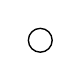
\begin{tikzpicture}[baseline=-1mm]\draw[fill=white,line width=0.5pt]  circle(1ex);\end{tikzpicture}称为``神经元''或者``节点''. 输入信号被送往神经元时, 会被分别乘以固定的权重$(x_1w_1,x_2w_2)$. 神经元会计算传送过来的信号的总和, 只有当这个总和超过了某个界限值时, 才会输出1. 这也称为``神经元被激活''. 这里将这个界限值称为\textbf{阈值}, 用符号$\theta$表示.

\begin{figure}
    \centering
    \scalebox{1}{
        \begin{tikzpicture}
            \begin{pgfonlayer}{nodelayer}
                \node [style=none] (0) at (1, 2) {};
                \node [style=none] (1) at (2, 2) {};
                \node [style=none] (2) at (1, 1) {};
                \node [style=none] (3) at (2, 1) {};
                \node [style=none] (4) at (1.5, 1.5) {$x_1$};
                \node [style=none] (5) at (1, 0) {};
                \node [style=none] (6) at (2, 0) {};
                \node [style=none] (7) at (1, -1) {};
                \node [style=none] (8) at (2, -1) {};
                \node [style=none] (9) at (1.5, -0.5) {$x_2$};
                \node [style=none] (10) at (4, 1) {};
                \node [style=none] (11) at (5, 1) {};
                \node [style=none] (12) at (4, 0) {};
                \node [style=none] (13) at (5, 0) {};
                \node [style=none] (14) at (4.5, 0.5) {$y$};
                \node [style=none] (15) at (2.25, 1.5) {};
                \node [style=none] (16) at (2.25, -0.5) {};
                \node [style=none] (17) at (3, 1.5) {$w_1$};
                \node [style=none] (18) at (3, -0.625) {$w_2$};
            \end{pgfonlayer}
            \begin{pgfonlayer}{edgelayer}
                \draw [bend left=45] (0.center) to (1.center);
                \draw [bend left=45] (1.center) to (3.center);
                \draw [bend left=45] (3.center) to (2.center);
                \draw [bend left=45] (2.center) to (0.center);
                \draw [bend left=45] (5.center) to (6.center);
                \draw [bend left=45] (6.center) to (8.center);
                \draw [bend left=45] (8.center) to (7.center);
                \draw [bend left=45] (7.center) to (5.center);
                \draw [bend left=45] (10.center) to (11.center);
                \draw [bend left=45] (11.center) to (13.center);
                \draw [bend left=45] (13.center) to (12.center);
                \draw [bend left=45] (12.center) to (10.center);
                \draw [style=diredge] (15.center) to (10.center);
                \draw [style=diredge] (16.center) to (12.center);
            \end{pgfonlayer}
        \end{tikzpicture}        
    }
    \caption{有两个输入的感知机}
\end{figure}

使用数学公式表示就是:

\begin{equation}
y = \begin{cases}
0, & \text{如果 } w_1x_1 + w_2x_2 \leq \theta \\
1, & \text{如果 } w_1x_1 + w_2x_2 > \theta
\end{cases}
\end{equation}

感知机的多个输入信号都有各自固有的权重, 这些权重发挥着控制各个信号的重要性的作用. 也就是说, 权重越大, 对应该权重的信号的重要性就越高.

\begin{note}
权重相当于电流里所说的电阻. 电阻是决定电流流动难度的参数, 电阻越低, 通过的电流就越大. 而感知机的权重则是值越大, 通过的信号就越大. 不管是电阻还是权重, 在控制信号流动难度(或者流动容易度)这一点上的作用都是一样的.
\end{note}

\section{简单逻辑电路}

\subsection{与门}

现在让我们考虑用感知机来解决简单的问题. 这里首先以逻辑电路为题材来思考一下与门(AND gate). 与门是有两个输入和一个输出的门电路. 图2-2这种输入信号和输出信号的对应表称为``真值表''. 如图2-2所示, 与门仅在两个输入均为1时输出1, 其他时候则输出0.

\begin{figure}
    \centering
    \scalebox{1}{
        \begin{tikzpicture}
            \begin{pgfonlayer}{nodelayer}
                \node [style=none] (0) at (1, 2) {$x_1$};
                \node [style=none] (1) at (3, 2) {$x_2$};
                \node [style=none] (2) at (4, 2) {$y$};
                \node [style=none] (3) at (1, 1) {$0$};
                \node [style=none] (4) at (3, 1) {$0$};
                \node [style=none] (5) at (4, 1) {$0$};
                \node [style=none] (6) at (1, 0) {$1$};
                \node [style=none] (7) at (3, 0) {$0$};
                \node [style=none] (8) at (4, 0) {$0$};
                \node [style=none] (9) at (1, -1) {$0$};
                \node [style=none] (10) at (3, -1) {$1$};
                \node [style=none] (11) at (4, -1) {$0$};
                \node [style=none] (12) at (1, -2) {$1$};
                \node [style=none] (13) at (3, -2) {$1$};
                \node [style=none] (14) at (4, -2) {$1$};
                \node [style=none] (15) at (0.5, 1.5) {};
                \node [style=none] (16) at (4.5, 1.5) {};
                \node [style=none] (17) at (3.5, 2.5) {};
                \node [style=none] (18) at (3.5, -2.5) {};
                \node [style=none] (19) at (0.5, 0.5) {};
                \node [style=none] (20) at (4.5, 0.5) {};
                \node [style=none] (21) at (0.5, -0.5) {};
                \node [style=none] (22) at (4.5, -0.5) {};
                \node [style=none] (23) at (0.5, -1.5) {};
                \node [style=none] (24) at (4.5, -1.5) {};
            \end{pgfonlayer}
            \begin{pgfonlayer}{edgelayer}
                \draw (15.center) to (16.center);
                \draw (17.center) to (18.center);
                \draw [style=box edge] (19.center) to (20.center);
                \draw [style=box edge] (21.center) to (22.center);
                \draw [style=box edge] (23.center) to (24.center);
            \end{pgfonlayer}
        \end{tikzpicture}        
    }
    \caption{与门的真值表}
\end{figure}

下面考虑用感知机来表示这个与门. 需要做的就是确定能满足图2-2的真值表的$w_1,w_2,\theta$的值. 那么, 设定什么样的值才能制作出满足图2-2的条件的感知机呢?

实际上, 满足图2-2的条件的参数的选择方法有无数多个. 比如, 当$(w_1,w_2,\theta)=(0.5,0.5,0.7)$时, 可以满足图2-2的条件. 此外, 当$(w_1,w_2,\theta)$为$(0.5, 0.5, 0.8)$或者$(1.0, 1.0, 1.0)$时, 同样也满足与门的条件. 设定这样的参数后, 仅当$x_1$和$x_2$同时为1时, 信号的加权总和才会超过给定的阈值$\theta$.

\subsection{与非门和或门}

接着, 我们再来考虑一下与非门(NAND gate). NAND 是 Not AND 的意思, 与非门就是颠倒了与门的输出. 用真值表表示的话, 如图 2-3 所示, 仅当$x_1$和$x_2$同时为1时输出0, 其他时候则输出1. 那么与非门的参数又可以是什么样的组合呢?

\begin{figure}
    \centering
    \scalebox{1}{
        \begin{tikzpicture}
            \begin{pgfonlayer}{nodelayer}
                \node [style=none] (0) at (1, 2) {$x_1$};
                \node [style=none] (1) at (3, 2) {$x_2$};
                \node [style=none] (2) at (4, 2) {$y$};
                \node [style=none] (3) at (1, 1) {$0$};
                \node [style=none] (4) at (3, 1) {$0$};
                \node [style=none] (5) at (4, 1) {$1$};
                \node [style=none] (6) at (1, 0) {$1$};
                \node [style=none] (7) at (3, 0) {$0$};
                \node [style=none] (8) at (4, 0) {$1$};
                \node [style=none] (9) at (1, -1) {$0$};
                \node [style=none] (10) at (3, -1) {$1$};
                \node [style=none] (11) at (4, -1) {$1$};
                \node [style=none] (12) at (1, -2) {$1$};
                \node [style=none] (13) at (3, -2) {$1$};
                \node [style=none] (14) at (4, -2) {$0$};
                \node [style=none] (15) at (0.5, 1.5) {};
                \node [style=none] (16) at (4.5, 1.5) {};
                \node [style=none] (17) at (3.5, 2.5) {};
                \node [style=none] (18) at (3.5, -2.5) {};
                \node [style=none] (19) at (0.5, 0.5) {};
                \node [style=none] (20) at (4.5, 0.5) {};
                \node [style=none] (21) at (0.5, -0.5) {};
                \node [style=none] (22) at (4.5, -0.5) {};
                \node [style=none] (23) at (0.5, -1.5) {};
                \node [style=none] (24) at (4.5, -1.5) {};
            \end{pgfonlayer}
            \begin{pgfonlayer}{edgelayer}
                \draw (15.center) to (16.center);
                \draw (17.center) to (18.center);
                \draw [style=box edge] (19.center) to (20.center);
                \draw [style=box edge] (21.center) to (22.center);
                \draw [style=box edge] (23.center) to (24.center);
            \end{pgfonlayer}
        \end{tikzpicture}        
    }
    \caption{与非门的真值表}
\end{figure}

要表示与非门, 可以用$(w_1,w_2,\theta)=(-0.5,-0.5,-0.7)$这样的组合(其他的组合也是无限存在的). 实际上, 只要把实现与门的参数值的符号取反, 就可以实现与非门.

接下来看一下图2-4所示的或门. 或门是``只要有一个输入信号是1, 输出就为1''的逻辑电路. 那么我们来思考一下, 应该为这个或门设定什么样的参数呢?

\begin{figure}
    \centering
    \scalebox{1}{
        \begin{tikzpicture}
            \begin{pgfonlayer}{nodelayer}
                \node [style=none] (0) at (1, 2) {$x_1$};
                \node [style=none] (1) at (3, 2) {$x_2$};
                \node [style=none] (2) at (4, 2) {$y$};
                \node [style=none] (3) at (1, 1) {$0$};
                \node [style=none] (4) at (3, 1) {$0$};
                \node [style=none] (5) at (4, 1) {$0$};
                \node [style=none] (6) at (1, 0) {$1$};
                \node [style=none] (7) at (3, 0) {$0$};
                \node [style=none] (8) at (4, 0) {$1$};
                \node [style=none] (9) at (1, -1) {$0$};
                \node [style=none] (10) at (3, -1) {$1$};
                \node [style=none] (11) at (4, -1) {$1$};
                \node [style=none] (12) at (1, -2) {$1$};
                \node [style=none] (13) at (3, -2) {$1$};
                \node [style=none] (14) at (4, -2) {$1$};
                \node [style=none] (15) at (0.5, 1.5) {};
                \node [style=none] (16) at (4.5, 1.5) {};
                \node [style=none] (17) at (3.5, 2.5) {};
                \node [style=none] (18) at (3.5, -2.5) {};
                \node [style=none] (19) at (0.5, 0.5) {};
                \node [style=none] (20) at (4.5, 0.5) {};
                \node [style=none] (21) at (0.5, -0.5) {};
                \node [style=none] (22) at (4.5, -0.5) {};
                \node [style=none] (23) at (0.5, -1.5) {};
                \node [style=none] (24) at (4.5, -1.5) {};
            \end{pgfonlayer}
            \begin{pgfonlayer}{edgelayer}
                \draw (15.center) to (16.center);
                \draw (17.center) to (18.center);
                \draw [style=box edge] (19.center) to (20.center);
                \draw [style=box edge] (21.center) to (22.center);
                \draw [style=box edge] (23.center) to (24.center);
            \end{pgfonlayer}
        \end{tikzpicture}        
    }
    \caption{或门的真值表}
\end{figure}

\begin{note}
这里决定感知机参数的并不是计算机, 而是我们人. 我们看着真值表这种``训练数据'', 人工考虑(想到)了参数的值. 而机器学习的课题就是将这个决定参数值的工作交由计算机自动进行. \textbf{学习}是确定合适的参数的过程, 而人要做的是思考感知机的构造(模型), 并把训练数据交给计算机.
\end{note}

如上所示, 我们已经知道使用感知机可以表示与门, 与非门, 或门的逻辑电路. 这里重要的一点是: 与门, 与非门, 或门的感知机构造是一样的. 实际上, 3个门电路只有参数的值(权重和阈值)不同. 也就是说, 相同构造的感知机, 只需通过适当地调整参数的值, 就可以像``变色龙演员''表演不同的角色一样, 变身为与门, 与非门, 或门.

\section{感知机的实现}

\subsection{简单的实现}

现在, 我们用Python来实现刚才的逻辑电路. 这里, 先定义一个接收参数x1和x2的AND函数.

\begin{mypython}
def AND(x1: float, x2: float) -> int:
    w1, w2, theta = 0.5, 0.5, 0.7
    tmp = x1 * w1 + x2 * w2
    if tmp <= theta:
        return 0
    else:
        return 1
\end{mypython}

在函数内初始化参数w1, w2, theta, 当输入的加权总和超过阈值时返回1, 否则返回0. 我们来确认一下输出结果是否如图2-2所示.

\begin{mypython}
AND(0, 0) # 输出0
AND(1, 0) # 输出0
AND(0, 1) # 输出0
AND(1, 1) # 输出1
\end{mypython}

果然和我们预想的输出一样! 这样我们就实现了与门. 按照同样的步骤, 也可以实现与非门和或门, 不过让我们来对它们的实现稍作修改.

\subsection{导入权重和偏置}

刚才的与门的实现比较直接, 容易理解, 但是考虑到以后的事情, 我们将其修改为另外一种实现形式. 在此之前, 首先把式(2.1)的$\theta$换成-b, 于是就可以用式(2.2)来表示感知机的行为.

\begin{equation}
y = \begin{cases}
0, & \text{如果 } b + w_1x_1 + w_2x_2 \leq \theta \\
1, & \text{如果 } b + w_1x_1 + w_2x_2 > \theta
\end{cases}
\end{equation}

式(2.1)和式(2.2)虽然有一个符号不同, 但表达的内容是完全相同的. 此处, b称为\textbf{偏置}, $w_1$和$w_2$称为\textbf{权重}. 如式(2.2)所示, 感知机会计算输入信号和权重的乘积, 然后加上偏置, 如果这个值大于0则输出1, 否则输出0. 下面, 我们使用NumPy, 按式(2.2)的方式实现感知机. 在这个过程中, 我们用Python的解释器逐一确认结果.

\begin{mypython}
>>> import numpy as np
>>> x = np.array([0, 1])
# 输入
>>> w = np.array([0.5, 0.5])
# 权重
>>> b = -0.7
# 偏置
>>> w*x
array([ 0. , 0.5])
>>> np.sum(w*x)
0.5
>>> np.sum(w*x) + b
-0.19999999999999996   # 大约为-0.2(由浮点数造成的运算误差)
\end{mypython}

如上例所示, 在NumPy数组的乘法运算中, 当两个数组的元素个数相同时, 各个元素分别相乘, 因此w*x的结果就是它们的各个元素分别相乘([0, 1] * [0.5, 0.5] => [0, 0.5]). 之后, np.sum(w*x)再计算相乘后的各个元素的总和. 最后再把偏置加到这个加权总和上, 就完成了式(2.2)的计算.

\subsection{使用权重和偏置的实现}

使用权重和偏置, 可以像下面这样实现与门.

\begin{mypython}
import numpy as np

def AND(x1: float, x2: float) -> int:
    x = np.array([x1, x2])
    w = np.array([0.5, 0.5])
    b = -0.7
    tmp = np.sum(w*x) + b
    if tmp <= 0:
       return 0
    else:
       return 1
\end{mypython}

这里把$-\theta$命名为偏置$b$, 但是请注意, 偏置和权重$w_1, w_2$的作用是不一样的. 具体地说, $w_1$和$w_2$是控制输入信号的重要性的参数, 而偏置是调整神经元被激活的容易程度(输出信号为$1$的程度)的参数. 比如, 若$b$为$-0.1$, 则只要输入信号的加权总和超过$0.1$, 神经元就会被激活. 但是如果$b$为$-20.0$, 则输入信号的加权总和必须超过$20.0$, 神经元才会被激活. 像这样, 偏置的值决定了神经元被激活的容易程度. 另外, 这里我们将$w_1$和$w_2$称为权重, 将$b$称为偏置, 但是根据上下文, 有时也会将$b,w_1,w_2$这些参数统称为权重.

接着, 我们继续实现与非门和或门.

\begin{mypythonhighlightlines}{3-4,13-14}
def NAND(x1, x2):
    x = np.array([x1, x2])
    w = np.array([-0.5, -0.5]) # 仅权重和偏置与AND不同!
    b = 0.7
    tmp = np.sum(w*x) + b
    if tmp <= 0:
        return 0
    else:
        return 1

def OR(x1, x2):
    x = np.array([x1, x2])
    w = np.array([0.5, 0.5]) # 仅权重和偏置与AND不同!
    b = -0.2
    tmp = np.sum(w*x) + b
    if tmp <= 0:
        return 0
    else:
        return 1
\end{mypythonhighlightlines}

我们在2.2节介绍过: 与门, 与非门, 或门是具有相同构造的感知机, 区别只在于权重参数的值. 因此, 在与非门和或门的实现中, 仅设置权重和偏置的值这一点和与门的实现不同.

\section{感知机的局限性}

到这里我们已经知道, 使用感知机可以实现与门, 与非门, 或门三种逻辑电路. 现在我们来考虑一下异或门(XOR gate).

\subsection{异或门}

异或门也被称为\textbf{逻辑异或}电路. 如图2-5所示, 仅当$x_1$或$x_2$中的一方为1时, 才会输出1(``异或''是拒绝其他的意思). 那么, 要用感知机实现这个异或门的话, 应该设定什么样的权重参数呢?

\begin{figure}
    \centering
    \scalebox{1}{
        \begin{tikzpicture}
            \begin{pgfonlayer}{nodelayer}
                \node [style=none] (0) at (1, 2) {$x_1$};
                \node [style=none] (1) at (3, 2) {$x_2$};
                \node [style=none] (2) at (4, 2) {$y$};
                \node [style=none] (3) at (1, 1) {$0$};
                \node [style=none] (4) at (3, 1) {$0$};
                \node [style=none] (5) at (4, 1) {$0$};
                \node [style=none] (6) at (1, 0) {$1$};
                \node [style=none] (7) at (3, 0) {$0$};
                \node [style=none] (8) at (4, 0) {$1$};
                \node [style=none] (9) at (1, -1) {$0$};
                \node [style=none] (10) at (3, -1) {$1$};
                \node [style=none] (11) at (4, -1) {$1$};
                \node [style=none] (12) at (1, -2) {$1$};
                \node [style=none] (13) at (3, -2) {$1$};
                \node [style=none] (14) at (4, -2) {$0$};
                \node [style=none] (15) at (0.5, 1.5) {};
                \node [style=none] (16) at (4.5, 1.5) {};
                \node [style=none] (17) at (3.5, 2.5) {};
                \node [style=none] (18) at (3.5, -2.5) {};
                \node [style=none] (19) at (0.5, 0.5) {};
                \node [style=none] (20) at (4.5, 0.5) {};
                \node [style=none] (21) at (0.5, -0.5) {};
                \node [style=none] (22) at (4.5, -0.5) {};
                \node [style=none] (23) at (0.5, -1.5) {};
                \node [style=none] (24) at (4.5, -1.5) {};
            \end{pgfonlayer}
            \begin{pgfonlayer}{edgelayer}
                \draw (15.center) to (16.center);
                \draw (17.center) to (18.center);
                \draw [style=box edge] (19.center) to (20.center);
                \draw [style=box edge] (21.center) to (22.center);
                \draw [style=box edge] (23.center) to (24.center);
            \end{pgfonlayer}
        \end{tikzpicture}        
    }
    \caption{异或门的真值表}
\end{figure}

实际上, 用前面介绍的感知机是无法实现这个异或门的. 为什么用感知机可以实现与门, 或门, 却无法实现异或门呢? 下面我们尝试通过画图来思考其中的原因.

首先, 我们试着将或门的动作形象化.

或门的情况下, 当权重参数$(b,w_1,w_2)=(-0.5,1.0,1.0)$时, 可满足图2-4的真值表条件. 此时, 感知机可用下面的式(2.3)表示.

\begin{equation}
y = \begin{cases}
0, & \text{如果\;} \text{-}0.5 + x_1 + x_2 \leq 0 \\
1, & \text{如果\;} \text{-}0.5 + x_1 + x_2 > 0
\end{cases}
\end{equation}

\begin{figure}
    \centering
    \scalebox{1}{
        \begin{tikzpicture}
            \begin{pgfonlayer}{nodelayer}
                \node [style=none] (0) at (0, 0) {};
                \node [style=none] (1) at (6, 0) {};
                \node [style=none] (2) at (2, -2) {};
                \node [style=none] (3) at (2, 4) {};
                \node [style=Z dot] (4) at (2, 0) {};
                \node [style=hadamard] (5) at (2, 2) {};
                \node [style=hadamard] (6) at (4, 2) {};
                \node [style=hadamard] (7) at (4, 0) {};
                \node [style=none] (11) at (1.5, -0.5) {$0$};
                \node [style=none] (12) at (2.5, 2.5) {$1$};
                \node [style=none] (13) at (4.5, -0.5) {$1$};
                \node [style=none] (14) at (6.5, 0) {$x_1$};
                \node [style=none] (15) at (2, 4.5) {$x_2$};
                \node [style=none] (16) at (-0.5, 3.5) {};
                \node [style=none] (17) at (5.5, -2.5) {};
                \node [style=none] (18) at (-0.5, -2.5) {};
            \end{pgfonlayer}
            \begin{pgfonlayer}{edgelayer}
                \draw [style=new edge style 0] (18.center)
                     to (17.center) [color=LightGray]
                     to (16.center)
                     to cycle;
                \draw [style=diredge] (0.center) to (1.center);
                \draw [style=diredge] (2.center) to (3.center);
                \draw [style=none] (16.center) to (17.center);
            \end{pgfonlayer}
        \end{tikzpicture}
    }
    \caption{感知机的可视化: 灰色区域是感知机输出$0$的区域, 这个区域与或门的性质一致}
\end{figure}

\begin{figure}
    \centering
    \scalebox{1}{
        \begin{tikzpicture}
            \begin{pgfonlayer}{nodelayer}
                \node [style=none] (0) at (0, 0) {};
                \node [style=none] (1) at (6, 0) {};
                \node [style=none] (2) at (2, -2) {};
                \node [style=none] (3) at (2, 4) {};
                \node [style=Z dot] (4) at (2, 0) {};
                \node [style=hadamard] (5) at (2, 2) {};
                \node [style=hadamard] (7) at (4, 0) {};
                \node [style=none] (11) at (1.5, -0.5) {$0$};
                \node [style=none] (12) at (2.5, 2.5) {$1$};
                \node [style=none] (13) at (4.5, -0.5) {$1$};
                \node [style=none] (14) at (6.5, 0) {$x_1$};
                \node [style=none] (15) at (2, 4.5) {$x_2$};
                \node [style=Z dot] (16) at (4, 2) {};
            \end{pgfonlayer}
            \begin{pgfonlayer}{edgelayer}
                \draw [style=diredge] (0.center) to (1.center);
                \draw [style=diredge] (2.center) to (3.center);
            \end{pgfonlayer}
        \end{tikzpicture}
    }
    \caption{圆形和正方形表示异或门的输出. 可否通过一条直线作出分割圆形和正方形的空间呢?}
\end{figure}

\begin{figure}
    \centering
    \scalebox{1}{
        \begin{tikzpicture}
            \begin{pgfonlayer}{nodelayer}
                \node [style=none] (17) at (0, 4) {};
                \node [style=none] (18) at (6.25, -2) {};
                \node [style=none] (19) at (6.25, 4) {};
                \node [style=none] (20) at (0.5, -1.5) {};
                \node [style=none] (22) at (1.5, -1.5) {};
                \node [style=none] (23) at (3.25, 0.5) {};
                \node [style=none] (24) at (5, 0.5) {};
                \node [style=none] (25) at (0.5, -0.75) {};
                \node [style=none] (26) at (3, 3.25) {};
                \node [style=none] (27) at (3, 1.5) {};
                \node [style=none] (0) at (0, 0) {};
                \node [style=none] (1) at (6, 0) {};
                \node [style=none] (2) at (2, -2) {};
                \node [style=none] (3) at (2, 4) {};
                \node [style=Z dot] (4) at (2, 0) {};
                \node [style=hadamard] (5) at (2, 2) {};
                \node [style=hadamard] (7) at (4, 0) {};
                \node [style=none] (11) at (1.5, -0.5) {$0$};
                \node [style=none] (12) at (2.5, 2.5) {$1$};
                \node [style=none] (13) at (4.5, -0.5) {$1$};
                \node [style=none] (14) at (6.5, 0) {$x_1$};
                \node [style=none] (15) at (2, 4.5) {$x_2$};
                \node [style=Z dot] (16) at (4, 2) {};
            \end{pgfonlayer}
            \begin{pgfonlayer}{edgelayer}
                \draw [style=new edge style 0] (26.center) [color=LightGray, draw=black]
                     to [bend left, looseness=1.25] (27.center)
                     to (25.center)
                     to [bend right=45, looseness=0.75] (20.center)
                     to [bend right, looseness=1.75] (22.center)
                     to [bend right=15, looseness=0.75] (23.center)
                     to [bend left] (24.center)
                     to [bend left=15] (18.center)
                     to (19.center)
                     to (17.center)
                     to [bend left=15] cycle;
                \draw [style=diredge] (2.center) to (3.center);
                \draw [style=diredge] (0.center) to (1.center);
                \draw [thick,draw=white] (6.25, -2.1) to (18.center) to (19.center);
                \draw [thick,draw=white] (17.center) to (19.center) to (6.25, 4.1);
            \end{pgfonlayer}
        \end{tikzpicture}        
    }
    \caption{使用曲线可以分开圆形和正方形}
\end{figure}

\begin{figure}
    \centering
    \scalebox{0.5}{
        \begin{tikzpicture}
            \begin{pgfonlayer}{nodelayer}
                \node [style=none] (0) at (-2, 3) {};
                \node [style=none] (1) at (0, 3) {};
                \node [style=none] (2) at (-2, 1) {};
                \node [style=none] (3) at (0, 1) {};
                \node [style=none] (4) at (-4, 2.5) {};
                \node [style=none] (5) at (-4, 1.5) {};
                \node [style=none] (6) at (-2, 2.5) {};
                \node [style=none] (7) at (-2, 1.5) {};
                \node [style=none] (8) at (1, 2) {};
                \node [style=none] (9) at (3, 2) {};
                \node [style=none] (10) at (6, 3) {};
                \node [style=none] (11) at (8, 3) {};
                \node [style=none] (12) at (6, 1) {};
                \node [style=none] (13) at (8, 1) {};
                \node [style=none] (14) at (4, 2.5) {};
                \node [style=none] (15) at (4, 1.5) {};
                \node [style=none] (16) at (6, 2.5) {};
                \node [style=none] (17) at (6, 1.5) {};
                \node [style=none] (18) at (9.475, 2) {};
                \node [style=none] (19) at (11, 2) {};
                \node [draw=black,circle,minimum height=5mm] (20) at (9.25, 2) {};
                \node [style=none] (21) at (14, 3) {};
                \node [style=none] (22) at (16, 3) {};
                \node [style=none] (23) at (14, 1) {};
                \node [style=none] (24) at (16, 1) {};
                \node [style=none] (25) at (12, 2.5) {};
                \node [style=none] (26) at (12, 1.5) {};
                \node [style=none] (27) at (14.7, 2.5) {};
                \node [style=none] (28) at (14.7, 1.5) {};
                \node [style=none] (29) at (17, 2) {};
                \node [style=none] (30) at (19, 2) {};
                \node [style=none] (31) at (-1.25, -0.5) {AND};
                \node [style=none] (32) at (7, -0.5) {NAND};
                \node [style=none] (33) at (15, -0.5) {OR};
            \end{pgfonlayer}
            \begin{pgfonlayer}{edgelayer}
                \draw (0.center) to (2.center);
                \draw (2.center) to (3.center);
                \draw [bend right=75, looseness=1.75] (3.center) to (1.center);
                \draw (1.center) to (0.center);
                \draw (4.center) to (6.center);
                \draw (5.center) to (7.center);
                \draw (8.center) to (9.center);
                \draw (10.center) to (12.center);
                \draw (12.center) to (13.center);
                \draw [bend right=75, looseness=1.75] (13.center) to (11.center);
                \draw (11.center) to (10.center);
                \draw (14.center) to (16.center);
                \draw (15.center) to (17.center);
                \draw (18.center) to (19.center);
                \draw [bend left=60, looseness=2.00] (21.center) to (23.center);
                \draw (23.center) to (24.center);
                \draw [bend right=75, looseness=1.75] (24.center) to (22.center);
                \draw (22.center) to (21.center);
                \draw (25.center) to (27.center);
                \draw (26.center) to (28.center);
                \draw (29.center) to (30.center);
            \end{pgfonlayer}
        \end{tikzpicture}        
    }
    \caption{与门, 与非门, 或门的符号}
\end{figure}

\begin{figure}
    \centering
    \scalebox{0.5}{
        \begin{tikzpicture}
            \begin{pgfonlayer}{nodelayer}
                \node [style=none] (8) at (15.25, 0) {};
                \node [style=none] (9) at (18.25, 0) {};
                \node [style=none] (10) at (6, 3) {};
                \node [style=none] (11) at (8, 3) {};
                \node [style=none] (12) at (6, 1) {};
                \node [style=none] (13) at (8, 1) {};
                \node [style=none] (14) at (2, 2.5) {};
                \node [style=none] (15) at (4, 1.5) {};
                \node [style=none] (16) at (6, 2.5) {};
                \node [style=none] (17) at (6, 1.5) {};
                \node [style=none] (25) at (3, -1.75) {};
                \node [style=none] (26) at (2, -2.75) {};
                \node [style=none] (27) at (5.95, -1.75) {};
                \node [style=none] (28) at (5.95, -2.75) {};
                \node [style=none] (29) at (13.25, 0.25) {};
                \node [style=none] (30) at (13.25, -0.25) {};
                \node [style=none] (31) at (8, -2.25) {};
                \node [style=none] (32) at (11.25, 1.75) {$s_1$};
                \node [style=none] (33) at (11.25, -1.5) {$s_2$};
                \node [style=none] (34) at (3, 2.5) {};
                \node [style=none] (35) at (4, -2.75) {};
                \node [style=none] (36) at (1, 2.5) {$x_1$};
                \node [style=none] (37) at (1, -2.75) {$x_2$};
                \node [style=none] (38) at (19, 0) {$y$};
                \node [style=none] (39) at (6, -1.25) {};
                \node [style=none] (40) at (8, -1.25) {};
                \node [style=none] (41) at (6, -3.25) {};
                \node [style=none] (42) at (8, -3.25) {};
                \node [style=none] (43) at (8, 2) {};
                \node [style=none] (44) at (13.25, 1) {};
                \node [style=none] (45) at (15.25, 1) {};
                \node [style=none] (46) at (13.25, -1) {};
                \node [style=none] (47) at (15.25, -1) {};
                \node [style=none] (48) at (7, 2) {?};
                \node [style=none] (49) at (7, -2.25) {?};
                \node [style=none] (50) at (14.25, 0) {?};
            \end{pgfonlayer}
            \begin{pgfonlayer}{edgelayer}
                \draw (8.center) to (9.center);
                \draw (14.center) to (16.center);
                \draw (15.center) to (17.center);
                \draw (25.center) to (27.center);
                \draw (26.center) to (28.center);
                \draw (31.center) to (30.center);
                \draw (34.center) to (25.center);
                \draw (15.center) to (35.center);
                \draw [style=new edge style 0] (13.center)
                     to (12.center)
                     to (10.center)
                     to (11.center)
                     to cycle;
                \draw [style=new edge style 0] (42.center)
                     to (41.center)
                     to (39.center)
                     to (40.center)
                     to cycle;
                \draw [style=new edge style 0] (43.center) to (29.center);
                \draw [style=new edge style 0] (47.center)
                     to (46.center)
                     to (44.center)
                     to (45.center)
                     to cycle;
            \end{pgfonlayer}
        \end{tikzpicture}        
    }
    \caption{将与门, 与非门, 或门代入到``?''中, 就可以实现异或门!}
\end{figure}

\begin{figure}
    \centering
    \scalebox{0.5}{
        \begin{tikzpicture}
            \begin{pgfonlayer}{nodelayer}
                \node [style=none] (0) at (13.25, 1) {};
                \node [style=none] (1) at (15.25, 1) {};
                \node [style=none] (2) at (13.25, -1) {};
                \node [style=none] (3) at (15.25, -1) {};
                \node [style=none] (8) at (16.25, 0) {};
                \node [style=none] (9) at (18.25, 0) {};
                \node [style=none] (10) at (6, 3) {};
                \node [style=none] (11) at (8, 3) {};
                \node [style=none] (12) at (6, 1) {};
                \node [style=none] (13) at (8, 1) {};
                \node [style=none] (14) at (2, 2.5) {};
                \node [style=none] (15) at (4, 1.5) {};
                \node [style=none] (16) at (6, 2.5) {};
                \node [style=none] (17) at (6, 1.5) {};
                \node [draw,circle,minimum height=5mm] (20) at (9.25, 2) {};
                \node [style=none] (21) at (6, -1.25) {};
                \node [style=none] (22) at (8, -1.25) {};
                \node [style=none] (23) at (6, -3.25) {};
                \node [style=none] (24) at (8, -3.25) {};
                \node [style=none] (25) at (3, -1.75) {};
                \node [style=none] (26) at (2, -2.75) {};
                \node [style=none] (27) at (6.7, -1.75) {};
                \node [style=none] (28) at (6.7, -2.75) {};
                \node [style=none] (29) at (13.25, 0.25) {};
                \node [style=none] (30) at (13.25, -0.25) {};
                \node [style=none] (31) at (9, -2.25) {};
                \node [style=none] (32) at (11.25, 1.75) {$s_1$};
                \node [style=none] (33) at (11.25, -1.5) {$s_2$};
                \node [style=none] (34) at (3, 2.5) {};
                \node [style=none] (35) at (4, -2.75) {};
                \node [style=none] (36) at (1, 2.5) {$x_1$};
                \node [style=none] (37) at (1, -2.75) {$x_2$};
                \node [style=none] (38) at (19, 0) {$y$};
            \end{pgfonlayer}
            \begin{pgfonlayer}{edgelayer}
                \draw (0.center) to (2.center);
                \draw (2.center) to (3.center);
                \draw [bend right=75, looseness=1.75] (3.center) to (1.center);
                \draw (1.center) to (0.center);
                \draw (8.center) to (9.center);
                \draw (10.center) to (12.center);
                \draw (12.center) to (13.center);
                \draw [bend right=75, looseness=1.75] (13.center) to (11.center);
                \draw (11.center) to (10.center);
                \draw (14.center) to (16.center);
                \draw (15.center) to (17.center);
                \draw [bend left=60, looseness=2.00] (21.center) to (23.center);
                \draw (23.center) to (24.center);
                \draw [bend right=75, looseness=1.75] (24.center) to (22.center);
                \draw (22.center) to (21.center);
                \draw (25.center) to (27.center);
                \draw (26.center) to (28.center);
                \draw (20) to (29.center);
                \draw (31.center) to (30.center);
                \draw (34.center) to (25.center);
                \draw (15.center) to (35.center);
            \end{pgfonlayer}
        \end{tikzpicture}        
    }
    \caption{通过组合与门, 与非门, 或门实现异或门}
\end{figure}

\begin{figure}
    \centering
    \scalebox{1}{
        \begin{tikzpicture}
            \begin{pgfonlayer}{nodelayer}
                \node [style=none] (0) at (1, 2) {$s_1$};
                \node [style=none] (1) at (3, 2) {$s_2$};
                \node [style=none] (2) at (4, 2) {$y$};
                \node [style=none] (3) at (1, 1) {$1$};
                \node [style=none] (4) at (3, 1) {$0$};
                \node [style=none] (5) at (4, 1) {$0$};
                \node [style=none] (6) at (1, 0) {$1$};
                \node [style=none] (7) at (3, 0) {$1$};
                \node [style=none] (8) at (4, 0) {$1$};
                \node [style=none] (9) at (1, -1) {$1$};
                \node [style=none] (10) at (3, -1) {$1$};
                \node [style=none] (11) at (4, -1) {$1$};
                \node [style=none] (12) at (1, -2) {$0$};
                \node [style=none] (13) at (3, -2) {$1$};
                \node [style=none] (14) at (4, -2) {$0$};
                \node [style=none] (15) at (-2.5, 1.5) {};
                \node [style=none] (16) at (4.5, 1.5) {};
                \node [style=none] (17) at (3.5, 2.5) {};
                \node [style=none] (18) at (3.5, -2.5) {};
                \node [style=none] (19) at (-2.5, 0.5) {};
                \node [style=none] (20) at (4.5, 0.5) {};
                \node [style=none] (21) at (-2.5, -0.5) {};
                \node [style=none] (22) at (4.5, -0.5) {};
                \node [style=none] (23) at (-2.5, -1.5) {};
                \node [style=none] (24) at (4.5, -1.5) {};
                \node [style=none] (25) at (0.5, 2.5) {};
                \node [style=none] (26) at (0.5, -2.5) {};
                \node [style=none] (27) at (-2, 1) {$0$};
                \node [style=none] (28) at (-0.5, 1) {$0$};
                \node [style=none] (29) at (-2, 0) {$1$};
                \node [style=none] (30) at (-0.5, 0) {$0$};
                \node [style=none] (31) at (-2, -1) {$0$};
                \node [style=none] (32) at (-0.5, -1) {$1$};
                \node [style=none] (33) at (-2, -2) {$1$};
                \node [style=none] (34) at (-0.5, -2) {$1$};
                \node [style=none] (35) at (-2, 2) {$x_1$};
                \node [style=none] (36) at (-0.5, 2) {$x_2$};
            \end{pgfonlayer}
            \begin{pgfonlayer}{edgelayer}
                \draw (15.center) to (16.center);
                \draw (17.center) to (18.center);
                \draw [style=box edge] (19.center) to (20.center);
                \draw [style=box edge] (21.center) to (22.center);
                \draw [style=box edge] (23.center) to (24.center);
                \draw (25.center) to (26.center);
            \end{pgfonlayer}
        \end{tikzpicture}        
    }
    \caption{异或门的真值表}
\end{figure}

\begin{figure}
    \centering
    \scalebox{1}{
        \begin{tikzpicture}
            \begin{pgfonlayer}{nodelayer}
                \node [style=none] (0) at (2.75, 2.5) {};
                \node [style=none] (1) at (3.75, 2.5) {};
                \node [style=none] (2) at (2.75, 1.5) {};
                \node [style=none] (3) at (3.75, 1.5) {};
                \node [style=none] (4) at (3.25, 2) {$x_1$};
                \node [style=none] (5) at (6.25, 2.5) {};
                \node [style=none] (6) at (7.25, 2.5) {};
                \node [style=none] (7) at (6.25, 1.5) {};
                \node [style=none] (8) at (7.25, 1.5) {};
                \node [style=none] (9) at (6.75, 2) {$s_1$};
                \node [style=none] (10) at (2.75, -0.25) {};
                \node [style=none] (11) at (3.75, -0.25) {};
                \node [style=none] (12) at (2.75, -1.25) {};
                \node [style=none] (13) at (3.75, -1.25) {};
                \node [style=none] (14) at (3.25, -0.75) {$x_2$};
                \node [style=none] (15) at (6.25, -0.25) {};
                \node [style=none] (16) at (7.25, -0.25) {};
                \node [style=none] (17) at (6.25, -1.25) {};
                \node [style=none] (18) at (7.25, -1.25) {};
                \node [style=none] (19) at (6.75, -0.75) {$s_2$};
                \node [style=none] (20) at (10, 1) {};
                \node [style=none] (21) at (11, 1) {};
                \node [style=none] (22) at (10, 0) {};
                \node [style=none] (23) at (11, 0) {};
                \node [style=none] (24) at (10.5, 0.5) {$y$};
                \node [style=none] (25) at (4, 2) {};
                \node [style=none] (26) at (6, 2) {};
                \node [style=none] (27) at (4, -0.75) {};
                \node [style=none] (28) at (6, -0.75) {};
                \node [style=none] (29) at (9.75, 0.5) {};
                \node [style=none] (30) at (7.5, 2) {};
                \node [style=none] (31) at (7.5, -0.75) {};
                \node [style=none] (32) at (3.25, 3.25) {第0层};
                \node [style=none] (33) at (6.75, 3.25) {第1层};
                \node [style=none] (34) at (10.5, 3.25) {第2层};
            \end{pgfonlayer}
            \begin{pgfonlayer}{edgelayer}
                \draw [bend left=45] (0.center) to (1.center);
                \draw [bend left=45] (1.center) to (3.center);
                \draw [bend left=45] (3.center) to (2.center);
                \draw [bend left=45] (2.center) to (0.center);
                \draw [bend left=45] (5.center) to (6.center);
                \draw [bend left=45] (6.center) to (8.center);
                \draw [bend left=45] (8.center) to (7.center);
                \draw [bend left=45] (7.center) to (5.center);
                \draw [bend left=45] (10.center) to (11.center);
                \draw [bend left=45] (11.center) to (13.center);
                \draw [bend left=45] (13.center) to (12.center);
                \draw [bend left=45] (12.center) to (10.center);
                \draw [bend left=45] (15.center) to (16.center);
                \draw [bend left=45] (16.center) to (18.center);
                \draw [bend left=45] (18.center) to (17.center);
                \draw [bend left=45] (17.center) to (15.center);
                \draw [bend left=45] (20.center) to (21.center);
                \draw [bend left=45] (21.center) to (23.center);
                \draw [bend left=45] (23.center) to (22.center);
                \draw [bend left=45] (22.center) to (20.center);
                \draw [style=diredge] (25.center) to (26.center);
                \draw [style=diredge] (27.center) to (28.center);
                \draw [style=diredge] (27.center) to (7.center);
                \draw [style=diredge] (25.center) to (15.center);
                \draw [style=diredge] (30.center) to (20.center);
                \draw [style=diredge] (31.center) to (22.center);
            \end{pgfonlayer}
        \end{tikzpicture}        
    }
    \caption{用感知机表示异或门}
\end{figure}

\section{多层感知机}

\section{从与非门到计算机}

\chapter{神经网络}

\section{从感知机到神经网络}

\section{激活函数}

\section{多维数组的运算}

\section{3层神经网络的实现}

\section{输出层的设计}

\section{手写数字识别}

\chapter{神经网络的学习}

\section{从数据中学习}

\section{损失函数}

\section{数值微分}

\section{梯度}

\section{学习算法的实现}

\chapter{误差反向传播法}

\section{计算图}

\section{链式法则}

\section{反向传播}

\section{简单层的实现}

\section{激活函数层的实现}

\section{Affine/Softmax层的实现}

\section{误差反向传播法的实现}

\chapter{与学习相关的技巧}

\section{参数的更新}

\section{权重的初始值}

\section{Batch Normalization}

\section{正则化}

\section{超参数的验证}

\chapter{卷积神经网络}

\section{整体结构}

\section{卷积层}

\section{池化层}

\section{卷积层和池化层的实现}

\section{CNN的实现}

\section{CNN的可视化}

\section{具有代表性的CNN}

\chapter{深度学习}

\section{加深网络}

\section{深度学习的小历史}

\section{深度学习的高速化}

\section{深度学习的应用案例}

\section{深度学习的未来}

\part{使用深度学习进行自然语言处理}

\chapter{自然语言和单词的分布式表示}

\section{什么是自然语言处理}

\section{同义词词典}

\section{基于计数的方法}

\section{基于计数的方法的改进}

\chapter{word2vec}

\section{基于推理的方法和神经网络}

\section{简单的word2vec}

\section{学习数据的准备}

\section{CBOW模型的实现}

\section{word2vec的补充说明}

\chapter{word2vec的高速化}

\section{word2vec的改进1}

\section{word2vec的改进2}

\section{改进版word2vec的学习}

\section{word2vec相关的其他话题}

\chapter{RNN}

\section{概率和语言模型}

\section{RNN}

\section{RNN的实现}

\section{处理时序数据的层的实现}

\section{RNNLM的学习和评价}

\chapter{Gated RNN}

\section{RNN的问题}

\section{梯度消失和LSTM}

\section{LSTM的实现}

\section{使用LSTM的语言模型}

\section{进一步改进RNNLM}

\chapter{基于RNN生成文本}

\section{使用语言模型生成文本}

\section{seq2seq模型}

\section{seq2seq的实现}

\section{seq2seq的改进}

\section{seq2seq的应用}

\chapter{Attention}

\section{Attention的结构}

\section{带Attention的seq2seq的实现}

\section{Attention的评价}

\section{关于Attention的其他话题}

\section{Attention的应用}

\part{自制类似PyTorch的深度学习框架}

\chapter{自动微分}

\chapter{用自然的代码表达}

\chapter{实现高阶导数}

\chapter{创建神经网络}

\chapter{高级挑战}

\part{PyTorch教程}

\part{Transformer时代: 变形金刚}

\chapter{Attention Is All You Need}

\section{注意力机制}

\section{编码器-解码器}

\section{残差连接和层归一化}

\chapter{使用PyTorch自己实现一个类GPT的模型}

\section{自注意力的代码实现}

\section{多头注意力的代码实现}

\section{模型的训练}

\chapter{预训练}

\section{什么是预训练}

\section{模型的微调}

\section{Hugging face简介}

Hugging face公司开源了10万个预训练模型.

虽然我们自己的电脑无法训练大模型, 但可以下载大模型, 然后输入特定的数据, 针对性的微调大模型供自己使用.

这样可以做到每个特定场景都有自己的大模型.

所以微调大模型的预训练工程师可能未来是一个点.

例如:

\begin{itemize}
    \item 针对gpt-2模型输入古诗词散文, 使这个大模型更精准的编写古诗词
    \item 针对gpt-2模型输入公司的客服风格的自然语言, 使这个大模型更准确的回复客户的问题
    \item 针对gpt-2模型输入带有公司风格的UI设计样稿, 是这个大模型更好的设计UI稿件
\end{itemize}

\part{项目实战}

\chapter{Bert模型精讲}

\section{使用PyTorch自己实现一个Bert模型}

\section{Bert模型的预训练和微调}

\chapter{使用Bert模型开发项目}

\section{使用Bert开发文本分类器}

\section{使用Bert开发基于知识图谱的问答系统}

\chapter{GPT模型精讲}

\section{优化之前使用PyTorch编写的类GPT的模型}

\section{GPT模型的预训练和微调}

\chapter{使用GPT模型开发项目}

\section{使用GPT开发自动写文章的文本生成器}

\part{强化学习}

GPT模型本质上是集大成的一个大模型. 融合了机器学习的三大流派: 符号主义(编译原理), 联结主义(神经网络)和控制论(强化学习).

\chapter{老虎机问题}

\chapter{马尔可夫决策过程}

\chapter{贝尔曼方程}

\chapter{动态规划}

\chapter{蒙特卡洛法}

\chapter{TD法}

\chapter{神经网络和Q学习}

\chapter{DQN}

\chapter{策略梯度法}

\chapter{未来}

\part{底层}

\chapter{C/C++教程}

\chapter{使用C语言实现神经网络}

\chapter{基于NVIDIA的CUDA接口的GPU编程}

\chapter{AI编译器}

将同一个深度学习模型编译并部署到不同异构芯片的编译器技术.

\part{机器学习方向的职业方向}

\chapter{算法工程师: 编写高性能低功耗的小模型满足小需求}

\chapter{预训练工程师: 预训练大模型, 将大模型改造成适合特定应用场景的大模型}

\chapter{机器学习系统工程师: 解决端到端的机器学习问题}

\chapter{AI编译器工程师}

\end{document}